%%%%%%%%%%%%%%%%%%%%%%%%%%%%%%%%%%%%%%%%%%%%%%%%%%
%%%%%%%%%%%%%%%%%%%%%%%%%%%
% paper on ecc2,3 in pp, pA, dA and He3A collisions
%%%%%%%%%%%%%%%%%%%%%%%%%%%%%%%%%%%%%%%%%%%%%%%%%%
%%%%%%%%%%%%%%%%%%%%%%%%%%%

\documentclass[preprint,showpacs,amsfonts,aps,prl,nofootinbib,floatfix]{revtex4}
%\documentclass[twocolumn,showpacs,amsfonts,aps,prc,nofootinbib,floatfix]{revtex4}
%\documentclass[twocolumn,showpacs,amsfonts,aps,prc,nofootinbib,floatfix,superscriptaddress]{revtex4}
%\documentclass[twocolumn,showpacs,amsfonts,aps,prc,floatfix,superscriptaddress]{revtex4}

%\voffset=5mm

\usepackage{mathrsfs}
\usepackage{epsfig}
\usepackage{amssymb}
\usepackage{amsfonts}
\usepackage{latexsym}
\usepackage{amsthm}

\usepackage{bm}
\usepackage{graphicx}
\usepackage{amsmath}
\usepackage{hyperref}
\usepackage{slashed}
\usepackage{caption}
\usepackage{epstopdf}

\usepackage{subcaption}
\usepackage{cleveref}
\captionsetup{compatibility=false}


\def\l{\left}
\def\r{\right}
\def\la{\langle}
\def\ra{\rangle}
\def\dla{\la\!\la}
\def\dra{\ra\!\ra}

\begin{document}

%%%%%%%%%%%%%%%%%%%%%%%%Front Matter%%%%%%%%%%%%%%%%%%%%
%%%%%%%%%%%%%%
%%%%%%%%%%%%%%%%%%%%%%%%%%%%%%%%%%%%%%%%%%%%%%%%%%
%%%%%%%%%%%%%%%%%%%%

\title{Initial state fluctuations in collisions between light and heavy ions} 


\author{Brian Baker}
\affiliation{Department of Physics, The Ohio State University,
  Columbus, Ohio 43210-1117, USA}
\author{Jordan Singer}
\affiliation{Department of Physics, The Ohio State University,
  Columbus, Ohio 43210-1117, USA}
\author{Kevin Welsh}
\affiliation{Department of Physics, The Ohio State University,
  Columbus, Ohio 43210-1117, USA}
\author{Ulrich Heinz}
\email[Correspond to\ ]{heinz.9@osu.edu}
\affiliation{Department of Physics, The Ohio State University,
  Columbus, Ohio 43210-1117, USA}
  
\begin{abstract}
blah blah \dots
\end{abstract}

\pacs{25.75.-q, 12.38.Mh, 25.75.Ld, 24.10.Nz}

\date{\today}

\maketitle

%%%%%%%%%%%%%%%%%%%%%%%%%%%%%%%%%%%%%%%%%%%%%%%%%%

\section{Introduction}
\label{sec1}
%%%%%%%%%%%%%%%%%%%%%%%%%%%%%%%%%%%%%%%%%%%%%%%%%%
%%%%%%%%%%%%%%%%%%%%%%%%%%%%%%%%%%%%%%%%%%%%%%%%%%
\section{Modeling the initial state of collisions between light and heavy ions}
\label{sec2}
%%%%%%%%%%%%%%%%%%%%%%%%%%%%%%%%%%%%%%%%%%%%%%%%%%
\subsection{Quantum fluctuations on the nucleon level}
\label{sec2a}
%%%%%%%%%%%%%%%%%%%%%%%%%%%%%%%%%%%%%%%%%%%%%%%%%%
%%%%%%%%%%%%%%%%%%%%%%%%%%%%%%%%%%%%%%%%%%%%%%%%%%
\subsubsection{Fluctuating nucleon positions}
\label{sec2a1}
To generate the initial configuration of the colliding nuclei, the Monte-Carlo Glauber model was used. For large nuclei, such as Au or Pb, the positions of their constituent nucleons are sampled from a Woods-Saxon distribution, imposing a hard-core radius (minimum inter-nucleon distance of 0.9fm [1]). With this generation scheme, a projectile proton is placed at position $(x_p,y_p)=(\frac{b}{2},0)$ in the transverse plane, where nucleus A is centered at position $(x_A,y_A)=(-\frac{b}{2},0)$. 
To generate a deuteron, our model first samples the relative nucleon separation according to the probability density obtained from the Hulthen wave function
\begin{align} 
\label{eq:HulthenPDF}
	P(r)&=4\pi r^2 |\Phi|^2\\
	\Phi(r)&=\sqrt{\frac{\alpha \beta(\alpha+\beta)}{2\pi(\alpha-\beta)^2}}\frac{e^{-\alpha r}-e^{-\beta r}}{r},
\end{align}
where $\alpha = 0.228$ fm$^{-1}$ and $\beta = 1.18$ fm$^{-1}$ (cite). Once the separation between the proton and neutron is sampled, the deuteron is given a random rotation in 3-space.
For the $^3$He and t nuclei, we used a set of 14,000 samplings of the positions of the three nucleons in these nuclei based on 3-body wave functions obtained from Green function Monte Carlo calculations using the AV18 + UIX model interaction \cite{Carlson:1997qn}. This set of 3-nucleon configurations was kindly provided by (...). After centering the 3-nucleon systems at $(x_t,y_t) = (\frac{b}{2},0)$, we orient the sampled $^3$He nuclei randomly in 3-space.

Nucleons in this model are described with a Gaussian probability distribution with a width controlled by the inelastic nucleon-nucleon cross-section $\sigma_{NN}^{inel}$. Projecting this Gaussian nucleon density distribution onto the transverse plane gives the nuclear thickness function \cite{Shen:2014vra}
\begin{equation} 
	T_{N}(r) = \frac{1}{(2\pi B)^2}e^{-\frac{r^2}{2B}},
\end{equation}

where the Gaussian width parameter B depends on collision energy, $\sqrt{s}$, through the inelastic nucleon-nucleon cross sections
\begin{equation}
	B(\sqrt{s}) = \frac{\sigma_{NN}^{inel}(\sqrt{s})}{14.30}
\end{equation}

This implementation differs from the popular choice of modeling the nucleons as cylindrical disks with axes along the beam direction by allowing, with small probability, inelastic collisions between nuclei that are separated by more than two mean nucleon radii in the transverse plane. Due to the nonzero tail of the nucleon shape, the average distance between two colliding nucleons is larger with our Gaussian shape than with the disk-like shape.  This has important consequences in the ellipticity of very peripheral p+Au and p+Pb collisions. For each projectile nucleon from nucleus A at transverse position $\vec{X}_{\perp i}$, we now compute its collision probability with any of the nucleons in the target B at position  $\vec{X}_{\perp j}$ as
\begin{equation}
	P_{ij} = (1-e^{-\sigma_{gg} T_{NN}(|\vec{X}_{\perp i}-\vec{X}_{\perp j}|)})_{i\in A, j\in B}
	\label{eq:CollisionProb}
\end{equation}
and vice versa. $\sigma_{gg}$ is the gluon-gluon cross section and $T_{NN}(b)$ is the nucleon-nucleon overlap function  \cite{Heinz:2011mh}

\begin{equation}
	\label{eq:NuclearOverlap}
	T_{NN}(b) = \int d^2 r_{\perp} T_{N}(\vec{r_{\perp}}) T_{N}(\vec{r}_{\perp}-\vec{b}) = \frac{e^{-\frac{b^2}{4B}}}{4\pi B}
\end{equation}

The nucleons (i,j) are labeled as “wounded” with probability $P_{ij}$. This procedure is performed on all pairs of projectile and target nucleons. No distinction is made between nucleons that suffered one or more inelastic collisions - all of them are labeled as “wounded”. For each wounded nucleon, i, we now assume that it deposits entropy density in the transverse plane with a Gaussian distribution 

\begin{equation}
	\sigma_{NN,i}(\vec{r}_{\perp}) = \frac{e^{-\frac{|\vec{r}_{\perp}-\vec{r}_{\perp,i}|^2}{2B}}}{2\pi B}
\end{equation}

The total initial entropy density at a given point in the transverse plane is then given by
\begin{equation}
	S_{o}(\vec{r}_{\perp}) = \sum\limits_{i=1}^{N_{w}} \frac{e^{-\frac{|\vec{r}_{\perp}-\vec{r}_{\perp,i}|^2}{2B}}}{2\pi B}
\end{equation}

where $N_{w}$ is the total number of wounded nucleons in the collision. 

%%%%%%%%%%%%%%%%%%%%%%%%%%%%%%%%%%%%%%%%%%%%%%%%%%
%%%%%%%%%%%%%%%%%%%%%%%%%%%%%%%%%%%%%%%%%%%%%%%%%%
\subsubsection{Nucleon-nucleon multiplicity fluctuations}
\label{sec2a2}

An entropy deposition model which assumes each nucleon deposits the same total entropy in the transverse plane fails to replicate the distribution of multiplicities observed in p+p collisions. To correct for this, the total entropy that each wounded nucleon deposits is allowed to vary by an overall factor $\gamma$. To best fit the observed distribution, $\gamma$ is sampled from a Gamma distribution
\begin{equation} 
	P(\gamma) = \frac{\gamma^{k-1} e^{-\frac{x}{\theta}}}{\theta^k \Gamma(k)}
\end{equation}
with shape parameter k and scale parameter $\theta$. This allows us to generate the new transverse entropy as
\begin{equation} 
	S_{o}(\vec{r}_{\perp}) = \sum\limits_{i=1}^{N_{w}} \gamma_{i} \frac{e^{-\frac{|\vec{r}_{\perp}-\vec{r}_{\perp,i}|^2}{2B}}}{2\pi B}
\end{equation}
This transverse entropy is then converted to the expected $\frac{dN_{ch}}{d\eta}$ from the collision by assuming they are linearly proportional
\begin{equation}
	\frac{dN_{ch}}{d\eta} = \frac{K_{s}}{\tau_0} * \frac{4.8*0.75}{8.9} \frac{dS}{dy}\biggr\rvert_{y=0} 
\end{equation}
Where $K_s$ is a factor used to match the observed mean multiplicity. To allow for statistical variance, the actual resulting multiplicity is sampled from a Poisson distribution with mean $\mu = \frac{dN_ch}{d\eta}$. To generate figure \ref{fig:pPbMultDist}, a sample of 500,000 p+Pb collisions at $\sqrt{s} = 5.02$ TeV were used. For each simulated event, the Poisson distribution was oversampled 5 times, resulting in 2.5 million data points. The choice for parameters $K_s$, and $\theta$ were taken from \cite{Shen:2014vra}.
\begin{figure}[!ht] 
	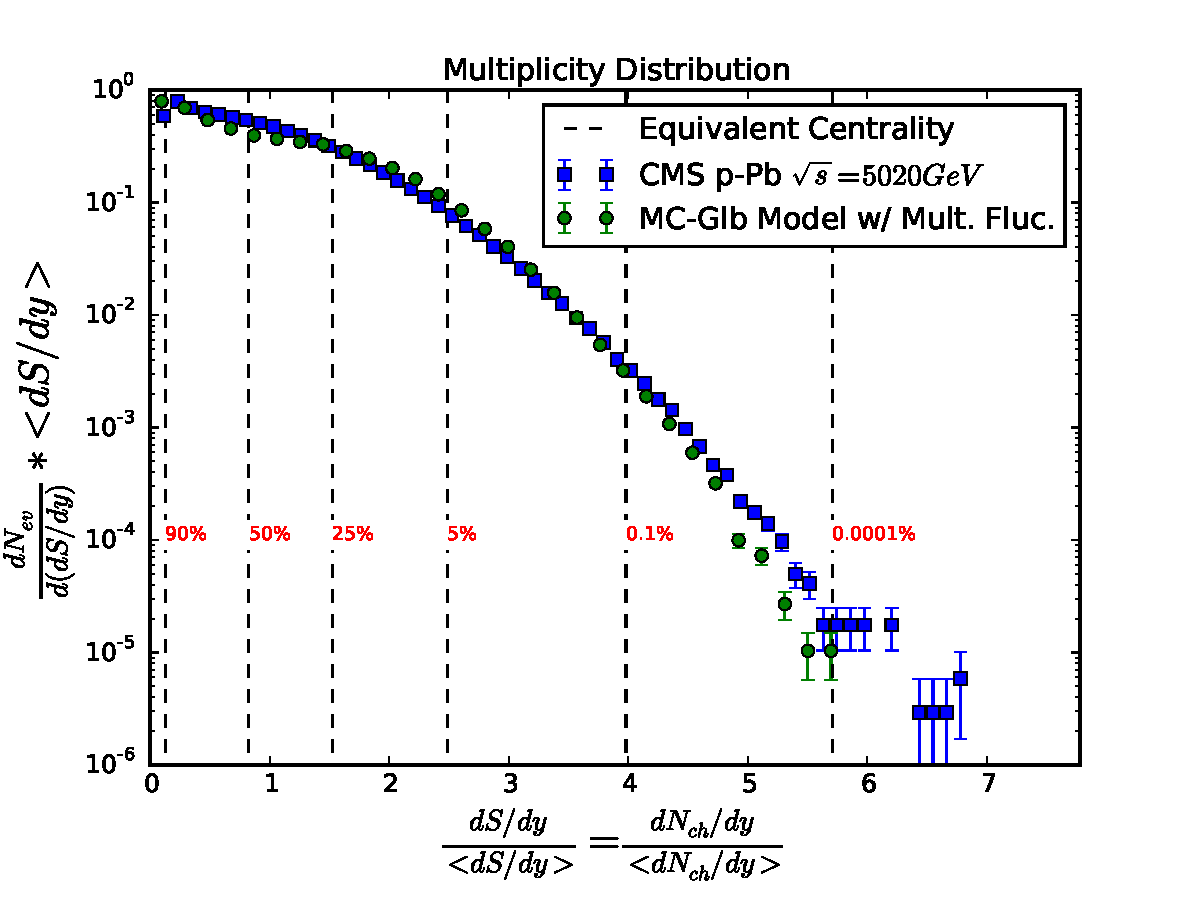
\includegraphics[width = \linewidth]{figs/TotalEntropyDist.pdf}
	\caption{Distribution of observed and simulated multiplicities assumed to be proportional to total entropy. Red numbers are estimates for centrality as determined from fraction of multiplicity. Fit parameters are $\theta=0.75$,$k=\frac{1}{\theta}=1.33$}
	\label{fig:pPbMultDist}
\end{figure}
%%%%%%%%%%%%%%%%%%%%%%%%%%%%%%%%%%%%%%%%%%%%%%%%%%
%%%%%%%%%%%%%%%%%%%%%%%%%%%%%%%%%%%%%%%%%%%%%%%%%%
\subsection{Quantum fluctuations on sub-nucleonic length scales}
\label{sec2b}
In heavy ion collisions, event-by-event fluctuations in nucleon position play a crucial role in determining anisotropies in the transverse entropy density distribution. However, light ion collisions show a larger dependency on smaller scale fluctuations in nucleon multiplicity and sub-nucleonic entropy density, due to fluctuations in the gluon field and valence quark positions.
%%%%%%%%%%%%%%%%%%%%%%%%%%%%%%%%%%%%%%%%%%%%%%%%%%
%%%%%%%%%%%%%%%%%%%%%%%%%%%%%%%%%%%%%%%%%%%%%%%%%%
\subsubsection{Quark subdivision of nucleons}
\label{sec2b1}
We suggest that a more physical model of a nucleon considers the positions of each valence quarks, and treats them as Gaussian gluon sources. To account for this, the positions of these quarks were randomly sampled from a Gaussian distribution about the center of the nucleon with width $\sqrt{B}$. The gluon density around these quarks was then modeled by a separate Gaussian distribution about each quark position with width $\sigma_g=0.2$fm. The effective width of the nucleon entropy deposition is 
\begin{equation} 
	\label{eq:QuarkConstraint}
	\sigma_{eff}^2 = \sigma_g ^2+B
\end{equation}
With quarks now providing the base Gaussian entropy density distribution, the multiplicity fluctuation factor $\gamma_q$ is sampled for and applied to the entropy density attributed to each quark.
\begin{equation} 
	\gamma_n = \sum_{i=1}^{3} \gamma_{qi}
\end{equation}
To maintain the same event-by-event multiplicity distribution, the PDF parameters must have the following relationships.
\begin{align}
	\theta_q &= \frac{\theta_n}{3}\\
	k_q &= \frac{1}{\theta_q} = 3 k_n
\end{align}
\begin{figure}[hb] 
	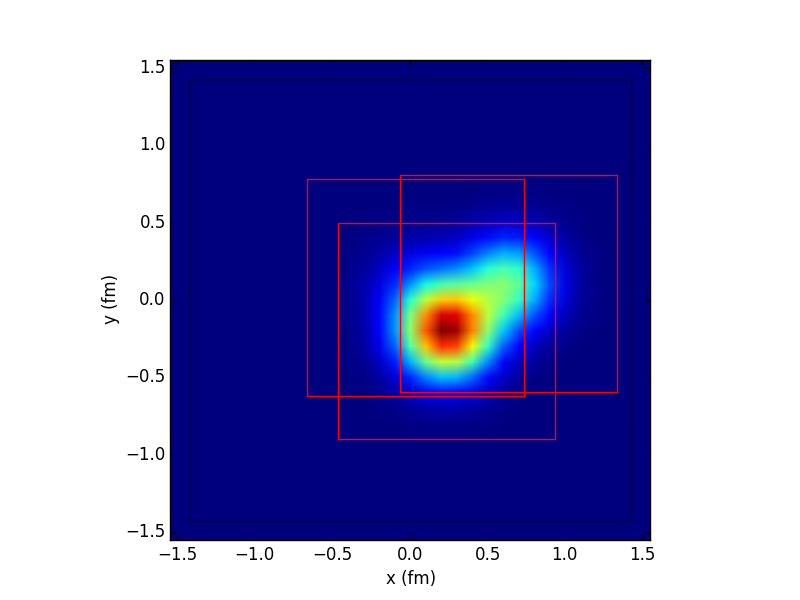
\includegraphics[width = 0.8\linewidth]{figs/QuarkSubstructure.png}
	\caption{Transverse entropy density distribution resulting from a p+p collision. The black box is the bounding box for the whole nucleon, which determines the cutoff for calculations. The red are bounding boxes are the same, for each quark. This addition of quark level detail allows for each nucleon to have an asymmetric, and in this case more triangular, structure when it otherwise would have no triangularity.}
	\label{fig:QuarkSubstructure}
\end{figure}
These considerations change the shape of the nuclear thickness function, $T_N(\vec{r})$, and the resultant transverse entropy deposition, $S_i(\vec{r}-\vec{r_i})$. The nuclear overlap function is no longer given by eq \ref{eq:CollisionProb}, but is now
\begin{equation}
	T_NN(\vec{b}) = \sum_{i=1}^{3}\sum_{j=1}^{3}\int{d^2r_\perp \frac{1}{4 \pi \sigma_g^2} e^{-\frac{(\vec{r}_{j\perp}+\vec{b}-\vec{r}_{i\perp})^2}{4 \sigma_g^2}}}
\end{equation}

Due to eq \ref{eq:QuarkConstraint}, the average nuclear thickness over many events approaches a Gaussian with a width $\sigma_{eff}$. This means that the average collision probability is still given by $P(i,j)$. However, since $T_{NN}(\vec{b})$ is only non-zero when the valence quarks overlap, certain configurations are biased when deciding wounded nucleons, which affects the measured eccentricities. Figure \ref{fig:CollisionComaprison} demonstrates this bias in p+p collisions at 200GeV.

\begin{figure}
	\label{fig:CollisionComaprison}
\end{figure}


%%%%%%%%%%%%%%%%%%%%%%%%%%%%%%%%%%%%%%%%%%%%%%%%%%
%%%%%%%%%%%%%%%%%%%%%%%%%%%%%%%%%%%%%%%%%%%%%%%%%%
\subsubsection{Sub-nucleonic gluon field fluctuations}
\label{sec2b2}
We introduce gluon field fluctuations in the entropy density of the wounded nucleons by first generating a Gamma distributed random field following the prescription of S. Moreland \cite{Moreland:2012qw}. We define the resulting distribution to be $\Gamma(\vec{r}_\perp)$. To apply the fluctuations, a large (30 fm by 30 fm) field was generated. For each nucleon $i$, a random square section is sampled from the grid with center $\vec{R_i}$ and width $10\sigma_p$.  The entropy density distribution of each nucleon is modified by 
\begin{equation}
	S'_{0i}(\vec{r}_\perp) = S_{0i}(\vec{r}_\perp) \Gamma(\vec{R_i} + \vec{r}_\perp) \Theta(5\sigma_p - |{\vec{R_i}-\vec{r_\perp}}|)
\end{equation}

%\begin{figure}[hb]
%	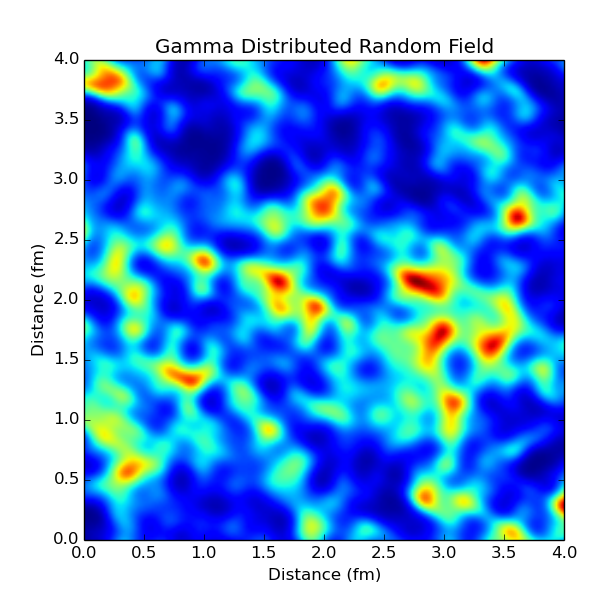
\includegraphics[width=.8\linewidth]{figs/GammaRandomField.png}
%	\caption{A small 4 fm x 4 fm sample section of the 100 fm x 100 fm Gamma random %field grid. The dark blue regions correspond to cold spots, where the entropy %density of the nucleons is decreased. The dark red regions correspond to hot spots, %where the entropy density of the nucleons is increased.}
%\end{figure} 
When the nucleons are modeled by a single smooth Gaussian, these small scale fluctuations have a noticeable effect on the resulting eccentricities. However, when they are applied to a nucleon represented with quark sub-structure, they have a negligible effect when considering collision probability and resulting eccentricity. Also, we argue that it is unreasonable to account for gluon field fluctuations when ignoring the much larger scale effect of quark position. As such, future analysis will omit this effect in both the smooth Gaussian and fluctuating quark structure cases.

%%%%%%%%%%%%%%%%%%%%%%%%%%%%%%%%%%%%%%%%%%%%%%%%%%
%%%%%%%%%%%%%%%%%%%%%%%%%%%%%%%%%%%%%%%%%%%%%%%%%%
\section{Results}
\label{sec:Results}
To examine the effects of fluctuations on the initial entropy density distribution, eccentricity is used as a measure of the deformity of a distribution. Of primary interest are the lower order eccentricities, $\epsilon_2$ and $\epsilon_3$, which are linearly proportional to the corresponding final state flow coefficients. These are defined by
\begin{align}
	\epsilon_n e^{i n\phi_n}& = -\frac{\int r dr d\phi r^n e^{i n \phi} \frac{d^2 S(r,\phi)}{dr d\phi}}{\int r dr d\phi r^2 \frac{d^2 S(r,\phi)}{dr d\phi}}\\
	\epsilon_n &\propto v_n, \forall n \in \{2,3\}
\end{align}

Unlike heavy ions, such as Au, light ions can exhibit intrinsic geometries that can bias certain eccentricities. For example, a deuteron only contains two nucleons, and as such, without sub-nucleonic fluctuations it is biased toward an elliptic deformation. Unfortunately, the influence that these intrinsic eccentricities have on the initial state anisotropies is not obvious. Figure \ref{fig:SmFlIntAu} shows the distribution of these intrinsic eccentricities found in deuterons and $^3$He nuclei with smooth Gaussian nucleons. Unintuitively, a $^3$He nucleus has a significantly larger elliptic eccentricity than the deuteron, despite the elliptic symmetry in the deuteron being so apparent. This is because the eccentricities are calculated in the transverse plane. While a deuteron is more loosely bound than $^3$He in 3-space, when projected onto the transverse plane it has a significantly smaller average intra-nuclear distance of 0.96 fm compared to ~1.8 fm as determined from eq \ref{eq:HulthenPDF}. Because a $^3$He nucleus contains 3 nucleons that are not co-linear, it will always have some elliptic deformation in the transverse plane, which is on average larger than a deuteron's. 
\begin{figure}
	\begin{center}
		\begin{subfigure}[t]{0.4\linewidth}
			%\centering
			\includegraphics[width = 1.12\textwidth] {figs/x_Au_200GeV/"Intrinsic_200GeV_Eccentricities_Deuteron,Helium3_Smooth".png}
			\subcaption{\label{subfig:SmIntAu}}
		\end{subfigure}
		\begin{subfigure}[t]{0.4\linewidth}
			%\centering
			\includegraphics[width = 1.12\textwidth] {figs/x_Au_200GeV/"Intrinsic_200GeV_Eccentricities_Deuteron,Helium3_Fluctuated".png}
			\subcaption{\label{subfig:FlIntAu}}
		\end{subfigure}
		\caption{\subref{subfig:SmIntAu} shows the eccentricity distribution for the intrinsic structure of the deuteron, and $^3$He. The smooth Gaussian proton is omitted, as its intrinsic entropy density is azimuthally symmetric. \subref{subfig:FlIntAu} shows the intrinsic eccentricity distributions when sub-nucleonic scale fluctuations are included. Since the quark sub-structure effectively replaces a proton with three smaller nucleons, one might expect that its profile would have a similar eccentricity to a $^3$He nucleus. However, since there is no quark-quark exclusion, the quarks more easily overlap in the transverse plane than the repulsive nucleons of $^3$He.}
		\label{fig:SmFlIntAu}
	\end{center}
\end{figure}

Naively, one would expect that these intrinsic geometries of light ions would appear in highly central collisions against a large nucleus, such as Au. However, figure \ref{fig:SmFlCentAu} shows evidence that intrinsic eccentricity is a poor predictor of low centrality eccentricities. This is largely due to two unintuitive effects in the collision modeling system. 

The first is the probabilistic binary collision detection method. Because the participation of two overlapping nucleons is determined by \ref{eq:CollisionProb}, the intrinsic geometry in the projectile nucleus is not guaranteed to carry over to the geometry of the wounded nucleons. Figure \ref{fig:SmFlAub=0} reveals that collision geometries at b = 0 bear little resemblance of the intrinsic nucleonic distributions, which gives additional credence to the above statement.

\begin{figure}
	\begin{center}
		\begin{subfigure}[t]{0.4\linewidth}
			%\centering
			\includegraphics[width = 1.12\textwidth] {figs/x_Au_200GeV/"Au_200GeV_Eccentricities_Deuteron,Helium3_Smooth_b=0".png}
			\subcaption{\label{subfig:SmAub=0}}
		\end{subfigure}
		\begin{subfigure}[t]{0.4\linewidth}
			%\centering
			\includegraphics[width = 1.12\textwidth] {figs/x_Au_200GeV/"Au_200GeV_Eccentricities_Deuteron,Helium3_Fluctuated_b=0".png}
			\subcaption{\label{subfig:FlAub=0}}
		\end{subfigure}
		\caption{\subref{subfig:SmAub=0} shows the eccentricity distribution for smooth Gaussian collisions at b = 0. \subref{subfig:FlAub=0} shows the eccentricity distributions when sub-nucleonic scale fluctuations are included, again at b = 0 collisions. }
		\label{fig:SmFlAub=0}
	\end{center}
\end{figure} 

Secondly, centrality is an unintuitive metric. The centrality for these collisions was calculated relative to the largest multiplicity found in that collision type \cite{Shen:2014vra}.
\begin{equation}
Centrality = \frac{1-\frac{dN_{ch}}{dy}}{Max(\frac{dN_{ch}}{dy})} 
\end{equation}
In heavy-ion collisions, it is reasonably correlated with impact parameter and $N_W$. However, in light-heavy collisions, this is not the case. Figures \ref{fig:MultVsNpart}, \ref{fig:NpartVsb} and \ref{fig:MultVsB} show that multiplicity, $N_W$ and impact parameter are only loosely correlated in light-heavy collisions. These correlations improve slightly as the size of the nuclei go up, but they are still poor in $^3$He+Au collisions.

\begin{figure}
	\includegraphics{figs/"MultiplicityVsNpart_p_Pb".png}
	\caption{}
	\label{fig:MultVsNpart}
\end{figure}

\begin{figure}
	\includegraphics{figs/"NpartVsb_p_Pb".png}
	\caption{}
	\label{fig:NpartVsb}
\end{figure}

\begin{figure}
	%\includegraphics{figs/"MultiplicityVsB".png}
	\caption{}
	\label{fig:MultVsB}
\end{figure}


\begin{figure}
	\centering
	\begin{subfigure}[h]{0.4\linewidth}
		\centering
		\includegraphics[width = 1.12\textwidth] {figs/x_Au_200Gev/"Au_200GeV_Eccentricities_Deuteron,Helium3_Smooth".png}
		\subcaption{\label{subfig:SmCentAu}}
	\end{subfigure}
	\begin{subfigure}[h]{0.4\linewidth}
		\centering
		\includegraphics[width = 1.12\textwidth] {figs/x_Au_200Gev/"Au_200GeV_Eccentricities_Deuteron,Helium3_Fluctuated".png}
		\subcaption{\label{subfig:FlCentAu}}
	\end{subfigure}
	\caption{Distributions of $\epsilon_2$ and $\epsilon_3$ found in x+Au collisions with low centrality (0-10\%). Neither with the smooth Gaussian model, \subref{subfig:SmCentAu}, nor with the added sub-nucleonic fluctuations, \subref{subfig:FlCentAu}, do the distributions resemble their intrinsic counterparts in FIG. 3.}
	\label{fig:SmFlCentAu}
\end{figure}


We have generated 500,000 MC-Glauber initial conditions for each collision type, x+Au at $\sqrt{s} = 200GeV$ and x+Pb at $\sqrt{s} = 5.02TeV$ where x $\in$ {p,d,$^3$He}. For each collision type, the eccentricities are plotted against centrality and impact parameter. Figure \ref{fig:AuENvsB} shows the event-averaged elliptic and triangular flows of x+Au collisions against impact parameter. It includes graphs data for both the smooth Gaussian case, and the fluctuated quark substructure case. Nucleons at this energy have a Gaussian width of 0.40 fm. Figure \ref{fig:PbENvsB} is the same, but with data from x+Pb collisions, where nucleons have a Gaussian width of 0.52 fm. In both, there are similar trends. In the low impact parameter range, 0-4 fm, each curve is relatively flat. This is because the light nucleus is entirely contained within the heavy nucleus. The p+A curves peak at large impact parameters, as the average nucleon separation gets larger. The black curves for the p+p collisions act as a reference to demonstrate that the eccentricity is highly sensitive to the distance between wounded nucleons. In the smooth case, the triangularity comes only from the multiplicity fluctuations, which break the reflectional symmetry. Even this small, not inherently triangular effect can produce a large $\epsilon_3$ when the wounded nucleons are spaced far enough away. This shows that while intrinsic geometry can bias certain eccentricities, other parameters, like average nucleon spacing, can be just as influential.
\begin{figure}[ht]
	\centering
	\includegraphics[width=\linewidth]{figs/x_Au_200GeV/"p,d,t+Au EN vs b".pdf}
	\caption{}
	\label{fig:AuENvsB}
\end{figure}
\begin{figure}
	\centering
	\includegraphics[width=\linewidth]{figs/x_Pb_5020GeV/"p,d,t+Pb EN vs b".pdf}
    \caption{\textbf{Eccentricities Vs. Impact Parameter:}  Shown are MC Glauber initial conditions for both RHIC (top) and LHC (bottom) for the elliptical and triangular eccentricities in p+Au, d+Au, and $^3$He+Au collisions as functions of impact parameter. In  (a) the entropy density for the collisions is deposited as a smooth Gaussian distribution, while in fig (b) the entropy profile is texturized with sub-nucleonic scale fluctuations. }
    \label{fig:PbENvsB}
\end{figure}
Figures \ref{fig:AuENvsCent} and \ref{fig:PbENvsCent} comprise our previous and updated expectations of experiments. They both show that the consideration of quark sub-structure has a large and complicated impact on initial state eccentricity. The most striking is that p, d and, $^3$He + A collisions now have very similar $\epsilon_3$ curves. When considering $^3$He+A collisions, one might expect that they would exhibit significantly higher $\epsilon_3$ at most, or all centralities. While this is the case with a smooth nucleon, the intrinsic geometry of $^3$He has a complicated manifestation when quarks are considered. Figure \ref{fig:PbENvsCent} even shows that $^3$He has the smallest $\epsilon_3$ from 30\%-70\%. This suggests that the random distribution of quarks washes out much of the small scale intrinsic geometry found in light ions. 

Because centrality is measured relative to the max $\frac{dN_{ch}}{dy}$ of each collision type, different centrality biases appear. For example, low centrality d+A collisions are correlated with a low impact parameter, but are biased toward a larger deuteron. This is because a larger deuteron will be able to hit more nucleons and generate a higher multiplicity. This is why we find a peak in the elliptic eccentricity at low centrality shown in figures \ref{fig:AuENvsCent} and \ref{fig:PbENvsCent}, but do not in figures \ref{fig:AuENvsB} and \ref{fig:PbENvsB}.
\begin{figure}[ht]
	\centering
	\includegraphics[width=\linewidth]{figs/x_Au_200GeV/"p,d,t+Au EN vs total_entropy".pdf}
	\caption{}
	\label{fig:AuENvsCent}
\end{figure} 
\begin{figure}[ht]
	\centering
	\includegraphics[width=\linewidth]{figs/x_Pb_5020GeV/"p,d,t+Pb EN vs total_entropy".pdf}
	\caption{\textbf{Eccentricities Vs. Centrality:} Centrality dependent eccentricities before (a) and after (b) the entropy density was texturized with sub-nucleonic fluctuations. Collisions were simulated for both RHIC (top) and LHC (bottom) energies}
	\label{fig:PbENvsCent}
\end{figure}

%%%%%%%%%%%%%%%%%%%%%%%%%%%%%%%%%%%%%%%%%%%%%%%%%%
\section{Summary and conclusions}
\label{sec5}
%%%%%%%%%%%%%%%%%%%%%%%%%%%%%%%%%%%%%%%%%%%%%%%%%%


\acknowledgments{We acknowledge fruitful and stimulating discussion with Jamie Nagle and thank Joe Carlson and Joel Lynn for providing us with 14,000 sampled nucleon configurations for $^3$He nuclei using state-of-the-art 3-nucleon wave functions. This work was supported by the U.S. Department of Energy, Office of Science, Office of Nuclear Physics under Awards No. \rm{DE-SC0004286} and (within the framework of the JET Collaboration) \rm{DE-SC0004104}. BB and KW gratefully acknowledge support through undergraduate summer research scholarships from the Department of Physics at The Ohio State University.}

%%%%%%%%%%%%%%% References %%%%%%%%%%%%%%%%%%%%%%%%%%%

%\bibliographystyle{h-physrev3}
%\bibliography{references}

\begin{thebibliography}{99}
	
%\cite{Carlson:1997qn}
\bibitem{Carlson:1997qn} 
J.~Carlson and R.~Schiavilla,
%``Structure and dynamics of few nucleon systems,''
Rev.\ Mod.\ Phys.\  {\bf 70}, 743 (1998).
%%CITATION = RMPHA,70,743;%%
%290 citations counted in INSPIRE as of 24 Apr 2015

%\cite{Heinz:2011mh}
\bibitem{Heinz:2011mh} 
U.~Heinz and J.~S.~Moreland,
%``Energy dependent growth of the nucleon and hydrodynamic initial conditions,''
Phys.\ Rev.\ C {\bf 84}, 054905 (2011)
[arXiv:1108.5379 [nucl-th]].
%%CITATION = ARXIV:1108.5379;%%
%11 citations counted in INSPIRE as of 14 Jul 2015

%\cite{Moreland:2012qw}
\bibitem{Moreland:2012qw} 
J.~S.~Moreland, Z.~Qiu and U.~W.~Heinz,
%``Imprinting Quantum Fluctuations on Hydrodynamic Initial Conditions,''
Nucl.\ Phys.\ A {\bf 904-905}, 815c (2013)
[arXiv:1210.5508 [nucl-th]].
%%CITATION = ARXIV:1210.5508;%%
%7 citations counted in INSPIRE as of 24 Apr 2015

%\cite{Nagle:2013lja}
\bibitem{Nagle:2013lja} 
J.~L.~Nagle, A.~Adare, S.~Beckman, T.~Koblesky, J.~O.~Koop, D.~McGlinchey, P.~Romatschke and J.~Carlson {\it et al.},
%``Exploiting Intrinsic Triangular Geometry in Relativistic He3+Au Collisions to Disentangle Medium Properties,''
Phys.\ Rev.\ Lett.\  {\bf 113}, no. 11, 112301 (2014)
[arXiv:1312.4565 [nucl-th]].
%%CITATION = ARXIV:1312.4565;%%
%25 citations counted in INSPIRE as of 24 Apr 2015

%\cite{Shen:2014vra}
\bibitem{Shen:2014vra} 
C.~Shen, Z.~Qiu, H.~Song, J.~Bernhard, S.~Bass and U.~Heinz,
%``The iEBE-VISHNU code package for relativistic heavy-ion collisions,''
arXiv:1409.8164 [nucl-th].
%%CITATION = ARXIV:1409.8164;%%
%14 citations counted in INSPIRE as of 24 Apr 2015
  

\end{thebibliography}

\end{document}

%%%%%%%%%%%% Extra references %%%%%%%%%%%%%%%%%%%%%%%%%%%%

\bibitem{Alver:2010dn} 
  B.~H.~Alver, C.~Gombeaud, M.~Luzum and J.-Y.~Ollitrault,
  %``Triangular flow in hydrodynamics and transport theory,''
  Phys.\ Rev.\ C {\bf 82}, 034913 (2010).
  %[arXiv:1007.5469 [nucl-th]].
  %%CITATION = ARXIV:1007.5469;%%  
  
\bibitem{Schenke:2011bn} 
  B.~Schenke, S.~Jeon and C.~Gale,
  %``Higher flow harmonics from (3+1)D event-by-event viscous hydrodynamics,''
  Phys.\ Rev.\ C {\bf 85}, 024901 (2012).
  %[arXiv:1109.6289 [hep-ph]].
  %%CITATION = ARXIV:1109.6289;%%
  
\bibitem{Muller:2006ee} 
  B.~M\"uller and J.~L.~Nagle,
  %``Results from the relativistic heavy ion collider,''
  Ann.\ Rev.\ Nucl.\ Part.\ Sci.\  {\bf 56}, 93 (2006).
  %[nucl-th/0602029].
  %%CITATION = NUCL-TH/0602029;%%  
  
\bibitem{Muller:2012zq} 
  B.~M\"uller, J.~Schukraft and B.~Wyslouch,
  %``First Results from Pb+Pb collisions at the LHC,''
  Ann.\ Rev.\ Nucl.\ Part.\ Sci.\  {\bf 62}, 361 (2012).
  %[arXiv:1202.3233 [hep-ex]].
  %%CITATION = ARXIV:1202.3233;%%  
  
\bibitem{Danielewicz:1984ww} 
  P.~Danielewicz and M.~Gyulassy,
  %``Dissipative Phenomena in Quark Gluon Plasmas,''
  Phys.\ Rev.\ D {\bf 31}, 53 (1985).
  %%CITATION = PHRVA,D31,53;%%  

\bibitem{Policastro:2001yc} 
  G.~Policastro, D.~T.~Son and A.~O.~Starinets,
  %``The Shear viscosity of strongly coupled N=4 supersymmetric Yang-Mills plasma,''
  Phys.\ Rev.\ Lett.\  {\bf 87}, 081601 (2001);
  %[hep-th/0104066].
  %%CITATION = HEP-TH/0104066;%%
%\bibitem{Kovtun:2004de} 
  P.~Kovtun, D.~T.~Son and A.~O.~Starinets,
  %``Viscosity in strongly interacting quantum field theories from black hole physics,''
  Phys.\ Rev.\ Lett.\  {\bf 94}, 111601 (2005).
  %[hep-th/0405231].
  %%CITATION = HEP-TH/0405231;%%  

\bibitem{Song:2010mg} 
  H.~Song, S.~A.~Bass, U.~Heinz, T.~Hirano and C.~Shen,
  %``200 A GeV Au+Au collisions serve a nearly perfect quark-gluon liquid,''
  Phys.\ Rev.\ Lett.\  {\bf 106}, 192301 (2011)
  [Erratum-ibid.\  {\bf 109}, 139904 (2012)].
  %[arXiv:1011.2783 [nucl-th]].
   
\bibitem{Luzum:2012wu} 
  M.~Luzum and J.-Y.~Ollitrault,
  %``Extracting the shear viscosity of the quark-gluon plasma from flow in ultra-central heavy-ion collisions,''
  Nucl.\ Phys.\ {\bf A904-905}, 377c (2013).
  %[arXiv:1210.6010 [nucl-th]].
  
\bibitem{Mishra:2007tw} 
  A.~P.~Mishra, R.~K.~Mohapatra, P.~S.~Saumia and A.~M.~Srivastava,
  %``Super-horizon fluctuations and acoustic oscillations in relativistic heavy-ion collisions,''
  Phys.\ Rev.\ C {\bf 77}, 064902 (2008);
  %[arXiv:0711.1323 [hep-ph]].
  %%CITATION = ARXIV:0711.1323;%%
%\bibitem{Mishra:2008dm} 
  %A.~P.~Mishra, R.~K.~Mohapatra, P.~S.~Saumia and A.~M.~Srivastava,
  %``Using cosmic microwave background radiation analysis tools for flow anisotropies in relativistic heavy-ion collisions,''
  and Phys.\ Rev.\ C {\bf 81}, 034903 (2010).
  %[arXiv:0811.0292 [hep-ph]].
  %%CITATION = ARXIV:0811.0292;%%  
  
\bibitem{Mocsy:2011xx} 
  A.~Mocsy and P.~Sorensen,
  %``Analyzing the Power Spectrum of the Little Bangs,''
  Nucl.\ Phys.\ A {\bf 855}, 241 (2011);
  %[arXiv:1101.1926 [hep-ph]].
  %%CITATION = ARXIV:1101.1926;%%  
%\bibitem{Sorensen:2011hm} 
  P.~Sorensen, B.~Bolliet, A.~Mocsy, Y.~Pandit and N.~Pruthi,
  %``The Rise and Fall of the Ridge in Heavy Ion Collisions,''
  Phys.\ Lett.\ B {\bf 705}, 71 (2011).
  %[arXiv:1102.1403 [nucl-th]].
  %%CITATION = ARXIV:1102.1403;%%
  
\bibitem{Heinz:2013wva} 
  U.~Heinz,
  %``Towards the Little Bang Standard Model,''
  J.\ Phys.\ Conf.\ Ser.\  {\bf 455}, 012044 (2013).
  %[arXiv:1304.3634 [nucl-th]].
  %%CITATION = ARXIV:1304.3634;%%
  
\bibitem{Staig:2010pn} 
  P.~Staig and E.~Shuryak,
  %``The Fate of the Initial State Fluctuations in Heavy Ion Collisions. II The Fluctuations and Sounds,''
  Phys.\ Rev.\ C {\bf 84}, 034908 (2011);
  %[arXiv:1008.3139 [nucl-th]].
  %%CITATION = ARXIV:1008.3139;%%  
%\bibitem{Staig:2011wj} 
  %P.~Staig and E.~Shuryak,
  %``The Fate of the Initial State Fluctuations in Heavy Ion Collisions. III The Second Act of Hydrodynamics,''
  Phys.\ Rev.\ C {\bf 84}, 044912 (2011);
  %[arXiv:1105.0676 [nucl-th]].
  %%CITATION = ARXIV:1105.0676;%%  
\bibitem{Shuryak:2013uaa} 
  E.~Shuryak and P.~Staig,
  %``The Sounds of the QCD Phase Transition,''
  Phys.\ Rev.\ C {\bf 88}, 064905 (2013).
  %[arXiv:1306.2938 [nucl-th]].
  %%CITATION = ARXIV:1306.2938;%%  
  
\bibitem{Lacey:2013is} 
  R.~A.~Lacey {\it et al.},
  %, Y.~Gu, X.~Gong, D.~Reynolds, N.~N.~Ajitanand, J.~M.~Alexander, A.~Mwai and A.~Taranenko,
  %``Is anisotropic flow really acoustic?,''
  arXiv:1301.0165 [nucl-ex];
  %%CITATION = ARXIV:1301.0165;%%  
%\bibitem{Lacey:2013qua} 
  %R.~A.~Lacey, A.~Taranenko, J.~Jia, D.~Reynolds, N.~N.~Ajitanand, J.~M.~Alexander, Y.~Gu and A.~Mwai,
  %``Beam entropy dependence of the viscous damping of anisotropic flow,''
  arXiv:1305.3341 [nucl-ex];
  %%CITATION = ARXIV:1305.3341;%%  
%\bibitem{Lacey:2013eia} 
  %R.~A.~Lacey {\it et al.},
  %, D.~Reynolds, A.~Taranenko, N.~N.~Ajitanand, J.~M.~Alexander, F.~-H.~Liu, Y.~Gu and A.~Mwai,
  %``Acoustic scaling of anisotropic flow in shape-engineered events: implications for extraction of the specific shear viscosity of the quark gluon plasma,''
  and arXiv:1311.1728 [nucl-ex].
  %%CITATION = ARXIV:1311.1728;%%  
 
\bibitem{CMS:2013bza} 
  S.~Chatrchyan {\it et al.}  [CMS Collaboration],
  %``Studies of azimuthal dihadron correlations in ultra-central PbPb collisions at $\sqrt{s_{NN}} =$ 2.76 TeV,''
  JHEP {\bf 1402}, 088 (2014)
  [arXiv:1312.1845 [nucl-ex]].
  %``Azimuthal anisotropy harmonics in ultra-central PbPb collisions at $\sqrt{s_\mathrm{NN}} = 2.76$\,TeV,''
  Physics Analysis Summary CMS-HIN-12-011, \url{http://cdsweb.cern.ch/record/1472724/files/HIN-12-011-pas.pdf}.

\bibitem{Luzum:2013yya} 
  M.~Luzum and H.~Petersen,
  %``Initial State Fluctuations and Final State Correlations in Relativistic Heavy-Ion Collisions,''
  J.\ Phys.\ G {\bf 41}, 063102 (2014)
  [arXiv:1312.5503 [nucl-th]].
  
\bibitem{Hirano:2009ah} 
  T.~Hirano and Y.~Nara,
  %``Eccentricity fluctuation effects on elliptic flow in relativistic heavy ion collisions,''
  Phys.\ Rev.\ C {\bf 79}, 064904 (2009)
  [arXiv:0904.4080 [nucl-th]].
  
\bibitem{Shen:2014vra} 
  C.~Shen, Z.~Qiu, H.~Song, J.~Bernhard, S.~Bass and U.~Heinz,
  %``The iEBE-VISHNU code package for relativistic heavy-ion collisions,''
  arXiv:1409.8164 [nucl-th]. 

\bibitem{Qiu:2012uy} 
  Z.~Qiu and U.~Heinz,
  %``Hydrodynamic event-plane correlations in Pb+Pb collisions at $\sqrt{s}=2.76$ATeV,''
  Phys.\ Lett.\ B {\bf 717}, 261 (2012)
  [arXiv:1208.1200 [nucl-th]].
  
\bibitem{Qiu:2011hf} 
  Z.~Qiu, C.~Shen and U.~Heinz,
  %``Hydrodynamic elliptic and triangular flow in Pb-Pb collisions at $\sqrt{s}=2.76$ATeV,''
  Phys.\ Lett.\ B {\bf 707}, 151 (2012)
  [arXiv:1110.3033 [nucl-th]].

\bibitem{Schenke:2012wb} 
  B.~Schenke, P.~Tribedy and R.~Venugopalan,
  %``Fluctuating Glasma initial conditions and flow in heavy ion collisions,''
  Phys.\ Rev.\ Lett.\  {\bf 108}, 252301 (2012)
  [arXiv:1202.6646 [nucl-th]].
     
\bibitem{Broniowski:2007nz} 
  W.~Broniowski, M.~Rybczynski and P.~Bozek,
  %``GLISSANDO: Glauber initial-state simulation and more..,''
  Comput.\ Phys.\ Commun.\  {\bf 180}, 69 (2009)
  [arXiv:0710.5731 [nucl-th]].

\bibitem{Qin:2010pf} 
  G.~Y.~Qin, H.~Petersen, S.~A.~Bass and B.~M\"uller,
  %``Translation of collision geometry fluctuations into momentum anisotropies in relativistic heavy-ion collisions,''
  Phys.\ Rev.\ C {\bf 82}, 064903 (2010);
  %[arXiv:1009.1847 [nucl-th]].
  %%CITATION = ARXIV:1009.1847;%% 
%\bibitem{Qin:2013bha} 
  G.~Y.~Qin and B.~M\"uller,
  %``Elliptic and triangular flow anisotropy in deuteron-gold collisions at $\sqrt{s_{NN}}=200$ GeV at RHIC and in proton-lead collisions at $\sqrt{s_{NN}}=5.02$ TeV at the LHC,''
  Phys.\ Rev.\ C {\bf 89}, 044902 (2014).
  %[arXiv:1306.3439 [nucl-th]].
  %%CITATION = ARXIV:1306.3439;%%  
 
\bibitem{Denicol:2014ywa} 
  G.~S.~Denicol, C.~Gale, S.~Jeon, J.-F.~Paquet and B.~Schenke,
  %``Effect of initial-state nucleon-nucleon correlations on collective flow in ultra-central heavy-ion collisions,''
  arXiv:1406.7792 [nucl-th].
  %%CITATION = ARXIV:1406.7792;%% 
  
\bibitem{Dumitru:2012yr} 
  A.~Dumitru and Y.~Nara,
  %``KNO scaling of fluctuations in pp and pA, and eccentricities in heavy-ion collisions,''
  Phys.\ Rev.\ C {\bf 85}, 034907 (2012)
  [arXiv:1201.6382 [nucl-th]].
  
\bibitem{Teaney:2010vd} 
  D.~Teaney and L.~Yan,
  %``Triangularity and Dipole Asymmetry in Heavy Ion Collisions,''
  Phys.\ Rev.\ C {\bf 83}, 064904 (2011)
  [arXiv:1010.1876 [nucl-th]].
  
 \bibitem{Qiu:2011iv} 
  Z.~Qiu and U.~Heinz,
  %``Event-by-event shape and flow fluctuations of relativistic heavy-ion collision fireballs,''
  Phys.\ Rev.\ C {\bf 84}, 024911 (2011).
  %[arXiv:1104.0650 [nucl-th]].

\bibitem{Gardim:2011xv} 
  F.~G.~Gardim, F.~Grassi, M.~Luzum and J.~Y.~Ollitrault,
  %``Mapping the hydrodynamic response to the initial geometry in heavy-ion collisions,''
  Phys.\ Rev.\ C {\bf 85}, 024908 (2012).
  %[arXiv:1111.6538 [nucl-th]].
  %%CITATION = ARXIV:1111.6538;%%
  
\bibitem{Teaney:2012ke} 
  D.~Teaney and L.~Yan,
  %``Non linearities in the harmonic spectrum of heavy ion collisions with ideal and viscous hydrodynamics,''
  Phys.\ Rev.\ C {\bf 86}, 044908 (2012).
  %[arXiv:1206.1905 [nucl-th]].
  %%CITATION = ARXIV:1206.1905;%%

 \bibitem{Mazeliauskas:2015vea} 
  A.~Mazeliauskas and D.~Teaney,
  %``Subleading harmonic flows in hydrodynamic simulations of heavy ion collisions,''
  arXiv:1501.03138 [nucl-th]. 
 
\bibitem{Rose:2014fba} 
  J.~B.~Rose, J.~F.~Paquet, G.~S.~Denicol, M.~Luzum, B.~Schenke, S.~Jeon and C.~Gale,
  %``Extracting the bulk viscosity of the quark-gluon plasma,''
  Nucl.\ Phys.\ A {\bf 931}, 926 (2014).
  %[arXiv:1408.0024 [nucl-th]].
  %%CITATION = ARXIV:1408.0024;%%

\bibitem{Lacey:2013qua} 
  R.~A.~Lacey, A.~Taranenko, J.~Jia, D.~Reynolds, N.~N.~Ajitanand, J.~M.~Alexander, Y.~Gu and A.~Mwai,
  %``Beam entropy dependence of the viscous damping of anisotropic flow in relativistic heavy ion collisions,''
  Phys.\ Rev.\ Lett.\  {\bf 112}, 082302 (2014).
  %[arXiv:1305.3341 [nucl-ex]].

\bibitem{Heinz:2013bua} 
  U.~Heinz, Z.~Qiu and C.~Shen,
  %``Fluctuating flow angles and anisotropic flow measurements,''
  Phys.\ Rev.\ C {\bf 87}, 034913 (2013).
  %[arXiv:1302.3535 [nucl-th]].
  
\bibitem{Aamodt:2011by} 
  K.~Aamodt {\it et al.}  [ALICE Collaboration],
  %``Harmonic decomposition of two-particle angular correlations in Pb-Pb collisions at $\sqrt{s_{NN}}=2.76$ TeV,''
  Phys.\ Lett.\ B {\bf 708}, 249 (2012).
  %[arXiv:1109.2501 [nucl-ex]].
  %%CITATION = ARXIV:1109.2501;%%  
    
\bibitem{Gardim:2012im} 
  F.~G.~Gardim, F.~Grassi, M.~Luzum and J.-Y.~Ollitrault,
  %``Breaking of factorization of two-particle correlations in hydrodynamics,''
  Phys.\ Rev.\ C {\bf 87}, 031901 (2013).
  %[arXiv:1211.0989 [nucl-th]].

\bibitem{Qiu:2012uy} 
  Z.~Qiu and U.~Heinz,
  %``Hydrodynamic event-plane correlations in Pb+Pb collisions at $\sqrt{s}=2.76$ATeV,''
  Phys.\ Lett.\ B {\bf 717}, 261 (2012).
  %[arXiv:1208.1200 [nucl-th]].

\bibitem{Schenke:2010rr} 
  B.~Schenke, S.~Jeon and C.~Gale,
  %``Elliptic and triangular flow in event-by-event (3+1)D viscous hydrodynamics,''
  Phys.\ Rev.\ Lett.\  {\bf 106}, 042301 (2011).
  %[arXiv:1009.3244 [hep-ph]].
  
\bibitem{Noronha-Hostler:2013gga} 
  J.~Noronha-Hostler, G.~S.~Denicol, J.~Noronha, R.~P.~G.~Andrade and F.~Grassi,
  %``Bulk Viscosity Effects in Event-by-Event Relativistic Hydrodynamics,''
  Phys.\ Rev.\ C {\bf 88}, 044916 (2013).
  %[arXiv:1305.1981 [nucl-th]].
  %%CITATION = ARXIV:1305.1981;%%  
  
\bibitem{ATLAS:2012at} 
  G.~Aad {\it et al.}  (ATLAS Collaboration),
  %``Measurement of the azimuthal anisotropy for charged particle production in $\sqrt{s_{NN}}=2.76$ TeV lead-lead collisions with the ATLAS detector,''
  Phys.\ Rev.\ C {\bf 86}, 014907 (2012).
  %[arXiv:1203.3087 [hep-ex]].
    
\bibitem{Qiu:2011hf} 
  Z.~Qiu, C.~Shen and U.~Heinz,
  %``Hydrodynamic elliptic and triangular flow in Pb-Pb collisions at $\sqrt{s}=2.76$ATeV,''
  Phys.\ Lett.\ B {\bf 707}, 151 (2012).
  %[arXiv:1110.3033 [nucl-th]].
  
\bibitem{Shen:2011eg} 
  C.~Shen, U.~Heinz, P.~Huovinen and H.~Song,
  %``Radial and elliptic flow in Pb+Pb collisions at the Large Hadron Collider from viscous hydrodynamics,''
  Phys.\ Rev.\ C {\bf 84}, 044903 (2011).
  %[arXiv:1105.3226 [nucl-th]].
  


  